
\subsection{A* Search Algorithm}
A* is a computer algorithm which is widely used to solve graph search problems \cite{a8book}. It determines the most efficient path between multiple nodes in a graph. A* is an informed search algorithm. This means, it searches between all the possible paths to the goal and finds the path incurring the least cost. To do this, it considers the paths which appear to have the least cost to get to the goal first. Starting from a specific node, it explores the graph step by step depending on the cost of going from one node to the next. The algorithm selects the node to explore based on a combination of the actual cost to get to the node and a heuristic cost that estimates the cost from the current node to the goal. The process to calculate heuristic cost is problem-specific. For the algorithm to work correctly, the heuristic cost has to be less than or equal to the actual cost of getting to the goal node. In other words, the heuristic cost function should never overestimate the cost of reaching the goal. The algorithm works by calculating the combined actual and heuristic cost for all the neighboring nodes of the starting node and puts them into a priority queue called the \textit{open list}. Then, it selects the node with the least cost and expands that node to get the cost of its neighbors. The expanded node is taken out of the priority queue and put in another list called the \textit{closed list}. The algorithm continues to expand the \textit{open list} always selecting the node with the least cost and adding it to the \textit{closed list}. The algorithm terminates when the goal node is inside the \textit{open list}, and it has the minimum cost in the \textit{open list}. Finally, the algorithm retraces its path through the \textit{closed list} to find the optimum route from start to goal. Pseudo code for the A* algorithm is given below.

\textbf{Algorithm 1:} A* search algorithm

\begin{algorithmic}[1]
\label{al:1}
% \Function{heuristic\_estimate}{$a,b$}
%     \State $hCost := \sum_{n=a}^b D(n)*R_{best}(n) $
%     \State \Return $hCost$
% \EndFunction

% \Function{gCost\_calc}{$p,c$}
%     \State $C_{actual}(pc) := C_{ESS}(pc)+C_{GRID}(t)+C_{best}(p)$
%     \State \Return $C_{actual}(pc)$
% \EndFunction

\Function{A*}{$start, goal$}
\State $Closed\_Set = \{\}$ \Comment{Set of evaluated nodes}
\State $Open\_Set = \{Start\}$ \Comment{Set of already discovered nodes which have not been evaluated. Initially,  the start node is discovered.}
\State $Best\_Parent[Start] = \{ \}$ \Comment{It is the node from which the current node can be most effectively reached. At initialization it is empty because the start node has no parent node.}
\State $F\_cost[Start] = G\_cost[Start] + H\_cost[Start]$ \Comment{$F\_cost$ is the combination of the actual cost of reaching a node from the start node \& the heuristic cost of reaching the goal node from the current node. $G\_cost$ is the actual cost \& $H\_cost$ is the heuristic cost of the current node. the Start node has a $G\_cost$ of $0$.}
\While{$Open\_Set$ is not empty}
    \State $Current\_Node = $ node in $Open\_Set$ with lowest $F\_cost$
    \If{$Current\_Node$ == goal}
      \State  \textbf{break} 
    \EndIf
    \For {Each child node of $Current\_Node$}
        \If{Child node in $Closed\_Set$}
            \State \textbf{continue}
        \EndIf
        \If{Child node in $Open\_Set$}
            \If{$G\_cost[child]$ $\geq$ $G\_cost$ already in $Open\_Set$}
                \State \textbf{continue}
            \EndIf
        \EndIf
        \State $Best\_Parent[child] = Current\_Node$
        \State $F\_cost[child] = G\_cost[child] + H\_cost[child]$
        \State $Open\_Set.add(child)$ \Comment{Add child node to $Open\_Set$}

    \EndFor
    \State $Closed\_Set.add(Current\_Node)$ \Comment{Add $Current\_Node$ to $Closed\_Set$}
    \State $Open\_Set.remove(Current\_Node)$ \Comment{Remove $Current\_Node$ From $Open\_Set$}
\EndWhile
\State $Best\_Path = \{ \}$ \Comment{$Best\_Path$ is the most efficient path to get to the goal node.}
\While{$Best\_Parent[Current\_Node] != \{ \}$}
    $Current\_Node = Best\_Parent[Current\_Node]$
    $Best\_Path.add(Current\_Node)$ \Comment{Add $Current\_Node$ to $Best\_Path$}
\EndWhile
\State \Return $Best\_Path$
\EndFunction
\end{algorithmic}


% Fig. \ref{fig:A_STAR_PIC} shows an example of the A* algorithm in a simple directional graph. The capital letters A, B, C, E, F, G and H inside the ellipses represent the nodes of the graph. The starting point of the graph is A, and the goal is to find the shortest path to node H. The solid blue arrows indicate the directional path from one node to the next. The actual cost of taking these paths are represented by the blue numbers beside the solid blue arrows. The red dotted lines represent the heuristic costs from a node to the target (goal) node. The heuristic costs of nodes B, C and G are shown as 7, 6 and 8. The letter 'h' is used to denote this cost. The algorithm starts at node A and discovers the surrounding nodes B and C. The combined heuristic and actual cost of node B is 9 and it is denoted by the letter 'f'. The 'f' cost for node C is 10. So, the algorithm will choose node B as the main candidate to explore. In node B, node E is discovered to have a combined cost of 10. Now, between the nodes C and E, the algorithm will choose a node at random. In this case, let us assume the node selected by the algorithm is E. After expanding E, the algorithm will find a path to node H which costs 10. However, this is still not the lowest path cost among all the nodes in the priority queue. C also has a cost of 10. So, the algorithm will expand the node C and discover two new nodes G and F. The combined heuristic and actual cost of node G is 15 and node F is 14, which in turn are more than 10. So, the algorithm will stop searching and decide that the shortest path from node A to H is the path previously discovered. By using this approach, A* lets us avoid exploring the nodes G and F because the combined heuristic and actual cost of a node are less than or equal to the actual cost taking a path through that node to the target.





% \begin{figure}[!ht]
% \centering
% %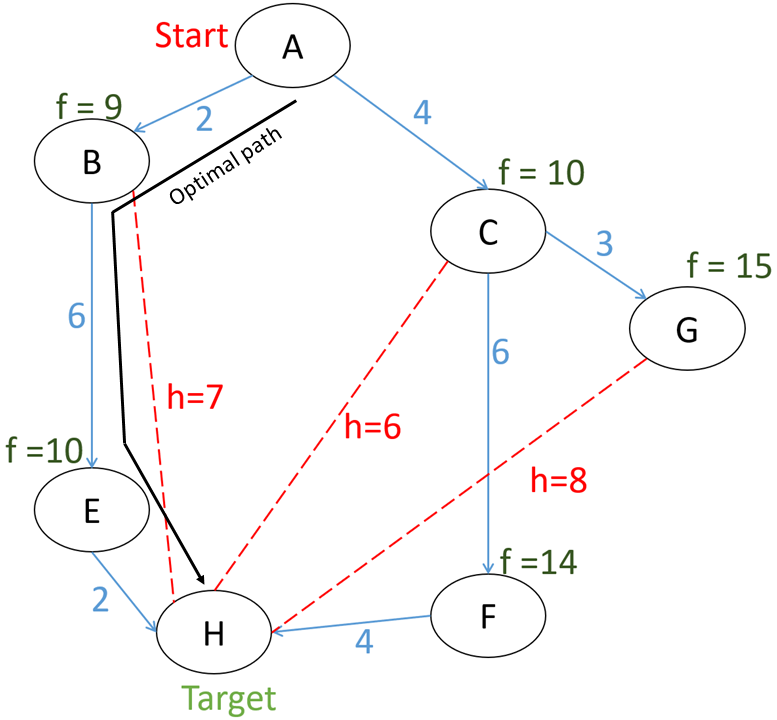
\includegraphics[width=\linewidth]{figs/A_STAR_PIC.png}
% 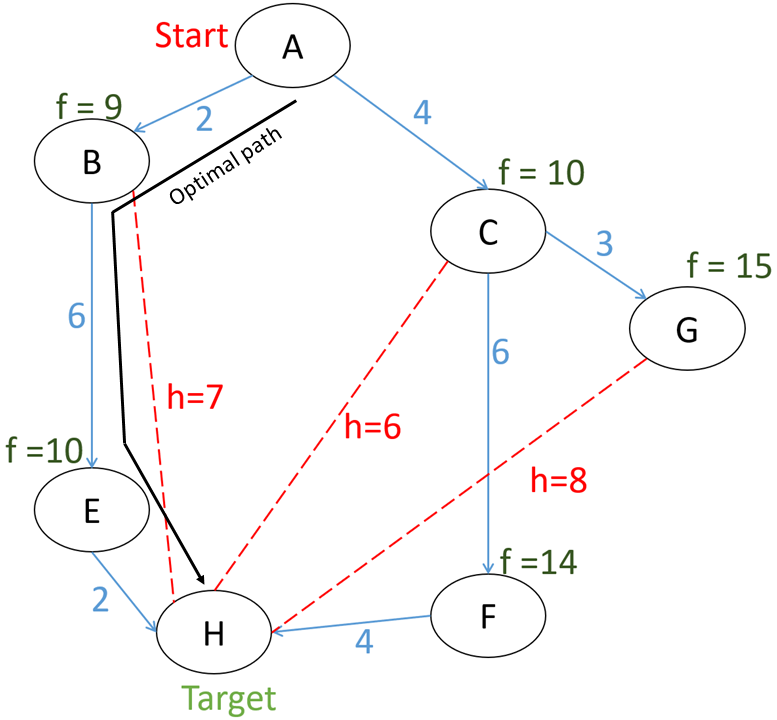
\includegraphics[width=\linewidth]{figs/A_STAR_PIC.png}
% \caption{Example graph for A* implementation}
% \label{fig:A_STAR_PIC}
% \end{figure}

\subsection{Implementation}
By defining the solution space with a combination of nodes and edges, the ESM optimization problem can be formulated as a graph search problem. At the inception, the starting node is determined by the current status of the system. Then, the following nodes and edges are generated using the forecasted data available. A discrete set of endpoints are set as the goals of the search. The A*  algorithm runs for all the goal nodes and the node with the lowest path cost is selected as the best end node.

The EMS recalculates the optimum path using the search algorithm at every time step based on updated information. The system status is assumed to be constant between time steps. The cost of going from a parent node to a child node is calculated by combining the real cost of getting to that child node and the heuristic cost of getting to the goal from that child node. The real cost of going from a parent node $p$ at time $T=t$ to a child node $c$ at time $T=t+\Delta T$ is denoted as $C_{actual}(pc)$. It is calculated according to (\ref{eq:C_actual}).

\begin{equation}
\label{eq:C_actual}
    C_{actual}(pc) =  C_{ESS}(pc)+C_{GRID}(t)+C_{best}(p)
\end{equation}

Here, $\Delta T$ represents the time between two time steps. $C_{actual}(pc)$ represent the total cost of going to the child node $c$ from parent node $p$. $C_{ESS}(pc)$ represent cost of energy storage to go from parent node $p$ to child node $c$. $C_{GRID}(t)$ is the cost of using the grid between time $T=t$ and time $T=t+\Delta T$. $C_{best}(p)$ represent the best or least cost to get to the parent node $p$ from the start node. $C_{ESS}(pc)$ is calculated according to (\ref{eq:C_ESS}).

\begin{equation}
\label{eq:C_ESS}
C_{ESS}(pc) = |(SOC_p - SOC_c)|*ESS_{CAP}*R_{ESS} 
\end{equation}

Here, $SOC_p$ and $SOC_c$ represent the state of charge at parent and child node. $ESS_{CAP}$ represent the total energy capacity of the energy storage. And $R_{ESS}$ is the $\$/kWh$ cost of using the energy storage. $C_{GRID}(t)$ is calculated according to (\ref{eq:C_GRID}).

\begin{equation}
\label{eq:C_GRID}
C_{GRID}(t) = 
\begin{cases}
   E_{GRID}(t)*RTP(t),& \text{if } E_{GRID}(t)\geq 0\\
    E_{GRID}(t)*SP(t),& \text{if }  E_{GRID}(t) < 0
\end{cases}
\end{equation}

Here, $E_{GRID}(t)$ is the energy drawn from the grid between time $T=t$ and time $T=t+\Delta T$. $RTP(t)$ is the real-time price between $t$ and $t+\Delta T$. $SP(t)$ is the price the utility is willing to pay the consumer for selling power between $t$ and $t+\Delta T$. The heuristic cost is calculated by assuming that whichever source has the smallest cost during a time step will supply the total energy demand of that particular time step. The heuristic cost of a node at time $T = t$ is calculated according to (\ref{eq:C_H}).

\begin{equation}
\label{eq:C_H}
C_H(t) = \sum_{n=t}^{end} D(n)*R_{best}(n)
\end{equation}

Here, $C_H(t)$ represents the heuristic cost at time $t$. $D(n)$ is the demand between time $T = n$ and time $T = n+\Delta T$. $R_{best}(n)$ is the source with the smaller cost which is calculated according to (\ref{eq:R_best}).

\begin{equation}
\label{eq:R_best}
R_{best}(n) = 
\begin{cases}
    R_{ESS},& \text{if } RTP(n)\geq R_{ESS}\\
    RTP(n),              & \text{otherwise}
\end{cases}
\end{equation}

After calculating the actual cost  $C_{actual}(pc)$ and heuristic cost $C_H(t)$, the total cost is finally calculated by adding  $C_{actual}(pc)$ and $C_H(t)$.

